\subsection{\techNew{}}
\label{sec:techc}
% \subsection{Data Locality in Micrographs}
\label{sec:technew}

%基于
\noindent
\zrdnew{
	\textbf{Observation III: }
	{Important token indices exhibit strong consistency across adjacent layers of an LLM.} To further analyze the distribution of important token indices, we examine the similarity of the top 25\% important token sets across adjacent layers for different models. As shown in Figure~\ref{fig:ob3}(a), there are two key observations: (1) the important tokens exhibit strong consistency across layers, and (2) tokens with higher importance in one layer are more likely to remain important in the subsequent layer.
	Specifically, xxxx.}
% 把图中的一些趋势或者例子挑出来说一下。

%
\begin{figure}
	\centering
	\subfigure[select the top 25\% most important tokens]{
		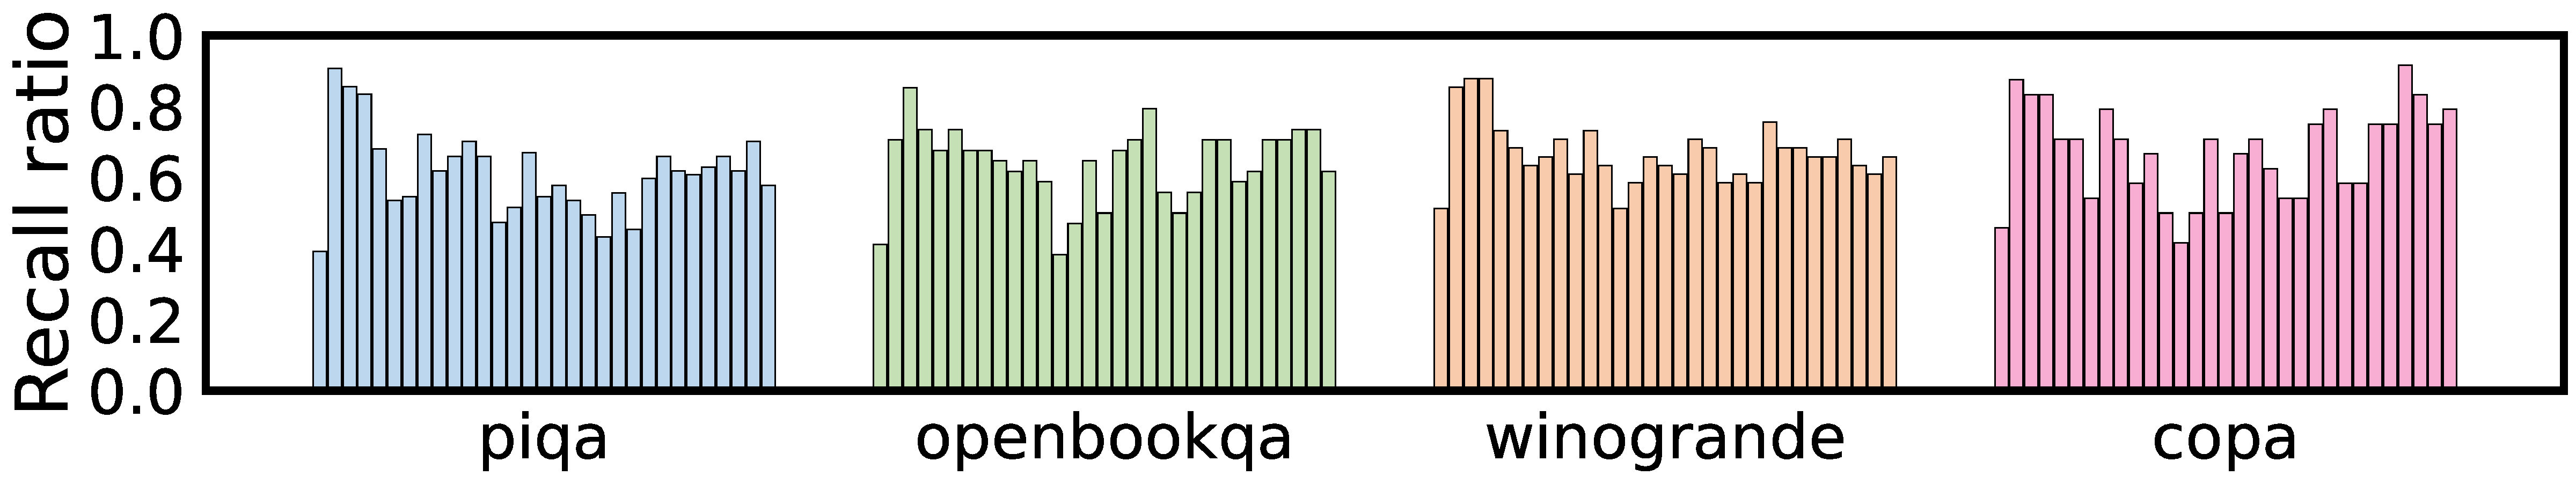
\includegraphics[width=1.5in, height=1in]{sim-25-cross-layers.pdf}
	}
	\subfigure[select different percentage most important tokens]{
		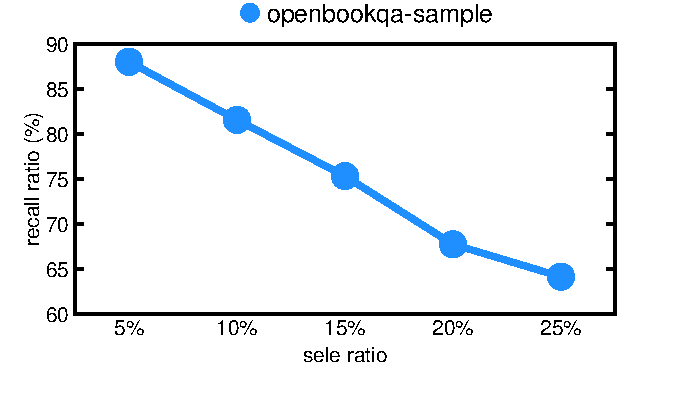
\includegraphics[width=1.5in, height=1in]{recall-sele.pdf}
	}
	\vspace{-0.1in}
	\caption{Similarities of important token index sets of adjacent layers.}
	\label{fig:ob3}
	\vspace{-0.1in}
\end{figure}
%如图xx所示,在模型的一层内,识别重要token index set和加载重要token的kv是有数据依赖的,在没有识别得到重要token index set的情况下,我们无法准确预取下一层所需的重要kv,因此在此层计算时,宝贵的I/O带宽没有被利用,在一个本就I/O瓶颈的场景下。一个naive的方法是,随机的预取一些下一层可能用到的token的kvs到GPU memory中,在下一层的重要token选择完成后,再把不在gpu mem的重要kv load到gpu mem中,然而这样的方法受制于完全不知道下一层重要token index的分布,准确率差,浪费了I/O带宽。一些工作提出了attention sink的概念,即一些特定位置的token在推理过程中总是重要的,如prompt的开头和结尾的几个token,然而,仅预取sink位置的token准确率仍不一定高(一些引用),且存在带宽利用不充分的可能。因此我们提出一种准确率高,灵活的指导预取的方法,高效的预取下一层的重要kv,并将预取与计算overlap起来。我们study了\cref{sec:techa}中提到的识别重要token的方法所识别出的重要token,发现在模型的相邻层重要token的分布是相似的,且重要性排名分位越靠前的index集合,相似度越高。相似度仍用jaccard index量化。
%图片xx描述了基于相似性的重要token识别方法识别出的,图片xx

%\zrdnew{For the important tokens identified as shown in Figure xx, within a given layer of the model, there exists a data dependency between identifying the important token index set and loading the corresponding prefix KVs. Without first identifying the important token index set, we are unable to accurately prefetch the necessary KVs for the next layer. As a result, valuable I/O bandwidth remains underutilized during computation in a scenario that is already constrained by I/O bottlenecks. A naive approach would be to randomly prefetch some potential KVs for the next layer into GPU memory. After the important token selection for the next layer is completed, any important KVs not already in GPU memory can then be loaded into it. However, this approach suffers from the challenge of not knowing the distribution of the important token index set for the next layer, resulting in low accuracy and wasted I/O bandwidth. Some works have proposed the concept of attention sinks, where certain tokens at specific positions, such as the beginning and end of a prompt, are always important during inference. However, prefetching only these sink tokens may still result in low accuracy (some references), and there is a risk of inefficient bandwidth utilization.}
%
%\zrdnew{To address these issues, we propose a more accurate and flexible guidance-based prefetching method that efficiently prefetches important KVs for the next layer while overlapping prefetching with computation. We studied the important tokens identified by the method mentioned in \cref{sec:techa} and found that the distribution of important tokens in adjacent layers is highly similar. Moreover, the index sets with higher importance rankings exhibit higher similarity. This similarity is quantified using the Jaccard index.}

\cp{
Loading important KVs during inference lies on the critical path and thus introduces non-negligible latency, as shown in Figure~\ref{}. 
To alleviate this overhead, we explore using prefetching to hide the I/O cost by overlapping data loading with computation. 
However, this presents a key challenge: the important tokens for the next transformer layer are unknown until the current layer’s computation completes, making it difficult to determine which KVs to prefetch in advance. 
To solve this challenge, based on \textit{Observation~III}, we propose the \technew{} mechanism, which exploits the strong similarity of important token index sets across adjacent layers. 
During the computation of the current layer, \technew{} asynchronously prefetches the important KVs of the next layer into GPU memory by approximating the next layer’s important tokens with those identified in the current layer. 
This layer-aware prefetching effectively reduces I/O latency and achieves higher accuracy than random prefetching.}


Existing LLM serving systems often face high inference latency due to inefficient KV management across GPU, CPU, and disk. 
Only KVs stored in GPU memory can be accessed with low latency, while fetching KVs from CPU or disk introduces substantial delay. 
These data transfers frequently occur on the critical path, causing I/O stalls, bandwidth underutilization, and longer time-to-first-token (TTFT). 


To address these issues, we propose an \textbf{importance-informed key–value (KV) prefetching system} with a \textbf{Dual Budget Strategy (DBS)} that jointly optimizes computation and I/O efficiency across heterogeneous storage tiers. 
Instead of merely overlapping data transfer with computation, our approach dynamically determines \emph{which} KVs to load and \emph{how much} I/O time to allocate to each storage tier within a fixed computation window $T_{\text{comp}}$. 
During each iteration, DBS prioritizes the KVs that yield the greatest accuracy improvement per unit of I/O cost and allocates separate time budgets for disk reads and PCIe transfers, ensuring that prefetching proceeds efficiently without exceeding the computational critical path.

Our system comprises two key components: (1) \textbf{importance-aware token prioritization} and (2) \textbf{dual-stage time budgeting}.  
First, each token is assigned an importance score $v(t)$ derived from its attention weight, while the cost of loading it from storage is estimated as $c(t) = c_{\text{disk}}(t) + c_{\text{pcie}}(t)$.  
We compute the ratio $\text{Density}(t) = v(t)/c(t)$ to evaluate how much benefit each unit of I/O time provides and greedily load tokens with the highest densities.  

Second, DBS partitions the computation time $T_{\text{comp}}$ into a disk I/O budget $T_{\text{disk}} = \rho_{\text{disk}}T_{\text{comp}}$ and a PCIe transfer budget $T_{\text{pcie}} = \rho_{\text{pcie}}T_{\text{comp}}$.  
Data are prefetched in a pipeline from disk to CPU and then to GPU, with dynamic budget adjustment to balance both stages and avoid idle time.  
Cached tokens incur negligible cost, while each disk access amortizes latency across multiple tokens, promoting sequential reads and improving throughput.  

Overall, this design minimizes redundant transfers, maximizes bandwidth utilization, and aligns prefetching time with computation, effectively reducing time-to-first-token (TTFT) without sacrificing inference accuracy.



	
%	Based on observation III, we propose the \technew{} mechanism.
%During the computation of the current layer, we  asynchronously prefetch important KVs of the next layer into GPU memory. This prefetching leverages the similarity of important token index sets across layers to improve prefetching accuracy. By approximating the important token index set of the next layer with the set from the current layer, we increase the accuracy of prefetching, leading to better performance compared to random prefetching. Once the important token index set for the next layer is identified, any important tokens' KVs that were not prefetched are then loaded into GPU memory for inference.


\zrdnew{To minimize inference latency in large language models (LLMs), we propose an importance-informed KV prefetching system that integrates a Dual Budget Strategy (DBS) to balance computation and I/O costs across heterogeneous storage tiers. During inference, key-value (KV) pairs are distributed among GPU, CPU, and disk, and the challenge lies in efficiently transferring the most important KVs to the GPU within a fixed computation time $T_{\text{comp}}$. Our design introduces two synergistic components: (1) **importance-aware token prioritization** and (2) **dual-stage time budgeting**. First, we quantify the importance of each token using the attention-based scores from the current layer and derive its expected value $v(t)$. The cost of loading a token $t$ from its storage location is estimated as $c(t) = c_{\text{disk}}(t) + c_{\text{pcie}}(t)$, where $c_{\text{disk}}(t) = \text{size(chunk)}/B_{\text{disk}}$ and $c_{\text{pcie}}(t) = \text{bytes}(t)/B_{\text{pcie}}$ represent the disk-read and PCIe-transfer times respectively. We then compute the **marginal density** $\text{Density}(t) = v(t)/c(t)$ and greedily select tokens with the highest density, ensuring that each unit of I/O time yields maximal contribution to model accuracy. Second, to achieve precise overlap between I/O and computation, we split the total time budget $T_{\text{comp}}$ into a **disk I/O budget** $T_{\text{disk}} = \rho_{\text{disk}}T_{\text{comp}}$ and a **PCIe transfer budget** $T_{\text{pcie}} = \rho_{\text{pcie}}T_{\text{comp}}$, where $\rho_{\text{disk}}$ and $\rho_{\text{pcie}}$ control the relative proportions of disk and PCIe utilization. Within each iteration, data are prefetched from disk to CPU and from CPU to GPU in a pipelined fashion, and dynamic adjustment of both budgets ensures that neither channel becomes idle or exceeds the computational critical path. Tokens already cached in GPU or CPU memory incur zero or partial cost, while the first access to a disk chunk amortizes the full read latency over multiple tokens, naturally encouraging dense, contiguous I/O. This design reduces redundant transfers, maximizes effective bandwidth, and guarantees that the prefetch time closely matches the computation time. The algorithm runs in $O(N\log N)$ time due to sorting by marginal density, with $O(N)$ space complexity. Ablation experiments compare the proposed DBS with static and random prefetching baselines under varying disk and PCIe bandwidths. Each experiment measures the time-to-first-token (TTFT), inference accuracy, and I/O efficiency. Specifically, we vary $\rho_{\text{disk}}$ and $\rho_{\text{pcie}}$ between 0.2 and 0.8 and evaluate scenarios where disk I/O or PCIe becomes the primary bottleneck. Experimental results demonstrate that DBS achieves up to 2.8× reduction in TTFT with negligible accuracy degradation (<0.2\%), confirming that balanced dual-stage budgeting and marginal density–based selection jointly maximize inference throughput under strict time constraints.}
